\documentclass{article}

\usepackage{caption}
\usepackage{subcaption}
\usepackage{amsmath}
\usepackage{url}

\usepackage{arxiv}

\usepackage[utf8]{inputenc} % allow utf-8 input
\usepackage[T1]{fontenc}    % use 8-bit T1 fonts
\usepackage{hyperref}       % hyperlinks
\usepackage{url}            % simple URL typesetting
\usepackage{booktabs}       % professional-quality tables
\usepackage{amsfonts}       % blackboard math symbols
\usepackage{nicefrac}       % compact symbols for 1/2, etc.
\usepackage{microtype}      % microtypography
\usepackage{lipsum}
\usepackage{graphicx}

\usepackage{algorithm}
\usepackage{algpseudocode}

\usepackage[backend=biber]{biblatex}
\addbibresource{refs.bib}

\graphicspath{ {./fig/} }

\usepackage{tikz}
\usetikzlibrary{arrows.meta, bending, positioning}

\newcommand{\txtop}[1]{\mathop{\mathrm{#1}}\limits}
\newcommand{\tanhl}{\txtop{tanh}}
\newcommand{\softmax}{\txtop{softmax}}
\newcommand{\linear}{\txtop{linear}}
\newcommand{\sigmoid}{\txtop{sigmoid}}
\newcommand{\DeePWAK}{\txtop{DeePWAK}}
\newcommand{\encoder}{\txtop{encoder}}
\newcommand{\decoder}{\txtop{decoder}}
\newcommand{\partitioner}{\txtop{partitioner}}

\date{\today}

\title{DeePWAK: Clustering \& Denoising Intertwined}

\author{Keira Wiechecki \\
  Center for Genomics \& Systems Biology \\
  New York University \\
	%\And 
        %Jade Zaslavsky
	%Lionel Christiaen \\
}

\begin{document}
\maketitle

\begin{abstract}
  Clustering is a special case of sparse dictionary learning where all features are discrete.
Here we introduce Denoising by Deep learning of a Partitoned Weighted Affinity Kernel (DeePWAK). 
\end{abstract}

\section{Introduction}
Though the applications of deep learning to classification is well established,

\subsection{noise2self}

Batson \& Royer\cite{batson2019noise2self} identify a class of denoising functions which can be optimised using only unlabeled noisy data.

Let $J \in \mathcal{J}$ be independent partitions of noisy data $X$. Let $\mathcal{F}(\theta)$ be a family of predictors of $X_J$ with tunable parameters $\theta \in \Theta$ that depends on its complement $X_{J^C}$

\begin{equation}
  \hat{X}_J=\mathcal{F}(\theta)(X_J^C)
\end{equation}

In other words, $\mathcal{F}$ predicts each data point $X_J$ from some subset of the data excluding $X_J$. 

  The optimal $\theta$ is given by

\begin{equation}
  \underset{\theta}{\overset{\Theta}{\mathrm{noise2self}}}[\mathcal{F}(\theta),X] := \underset{\theta}{\overset{\Theta}{\mathrm{argmin}}}[\sum_{J}^{\mathcal{J}}\mathbb{E}||X_J-\mathcal{F}(\theta)(X_{J^C})||^2]
\end{equation}



\subsection{Graph diffusion}

Our choice of $\mathcal{F}$ is adapted from DEWAKSS\cite{tjarnberg2021}. The parameters we want to tune generate a graph $G$ from embeddings $E$. The adjacency matrix of any graph can be treated as a transition matrix (or weighted affinity kernel) by setting the diagonal to 0 and normalizing columns to sum to 1. We call this the $\mathrm{WAK}$ function. For each embedding, an estimate is calculated based on its neighbors in the graph. This can be expressed as matrix multiplication.

\begin{equation}
\hat{E} := \mathrm{WAK}(G)E^\top
\end{equation}

Though DEWAKSS uses a $k$-NN graph, any adjacency matrix will do.
A clustering can be expressed as a graph where points within a cluster are completely connected and clusters are disconnected.

Let $C^{c \times n}$ be a matrix representing a clustering of $n$ points into $c$ clusters. Let each column be a 1-hot encoding of a cluster assignment for each point. We can obtain a partition matrix $P^{n \times n}$ by

\begin{equation}
  P := C^\top C
\end{equation}

\section{Notation}
Capital letters indicate matrices. Subscripts indicate indices. Superscripts indicate dimensionality. A circumflex indicates a reconstruction of data by a predictor. Lowercase Greek letters indicate tunable parameters. Capital Greek letters indicate parameter spaces. For parameters $\theta$, $\theta^{m \to d}$ indicates parameters for a model that accepts an input of dimension $m$ and returns an output of dimension $d$.

\section{Architecture}

The DeePWAK constructor has the type signature

\begin{equation}
  \mathrm{DeePWAK} := \forall m,d,c :\mathbb{N} \to (\mathbb{R}^m \to \mathbb{R}^d) \to (\mathbb{R}^m \to \mathbb{R}^c) \to (\mathbb{R}^d \to \mathbb{R}^m) \to \mathbb{R}^m \to \mathbb{R}^m
\end{equation}

It consists of an encoder, partitioner, and decoder.

\begin{algorithm}
  \caption{DeePWAK constructor}\label{alg:cap}
  \begin{algorithmic}[1]
    \State \textbf{data} $\mathrm{DeePWAK}${
    \State $\mathrm{encoder} : \exists m,d : \mathbb{N} \to \mathbb{R}^m \to \mathbb{R}^d$
    \State $\mathrm{partitioner} : \exists m,c : \mathbb{N} \to \mathbb{R}^m \to \mathbb{R}^c$
    \State $\mathrm{decoder} : \exists d,m : \mathbb{N} \to \mathbb{R}^d \to \mathbb{R}^m$
    }
  \end{algorithmic}
\end{algorithm}

\begin{algorithm}
  \caption{DeePWAK application}\label{alg:cap}
  \begin{algorithmic}[1]
    \State \textbf{function} $\mathrm{DeePWAK}(\theta, \pi, \phi)(X : \mathbb{R}^{m \times n})${
    \State $E \gets \theta(X)$
    \State $C \gets (\mathrm{softmax} \circ \pi)(X)$
    \State $P \gets C^\top C$
    \State $G \gets \mathrm{WAK}(P)$
    \State $\hat{E} \gets (GE^\top)^\top$
    \State $\hat{X} \gets \phi(\hat{E})$
    \State \textbf{return} $\hat{X}$
    }
  \end{algorithmic}
\end{algorithm}

\subsection{Multihead DeePWAK}

\section{A concrete example from microscopy data}

\begin{figure}
     \begin{subfigure}[b]{0.45\textwidth}
        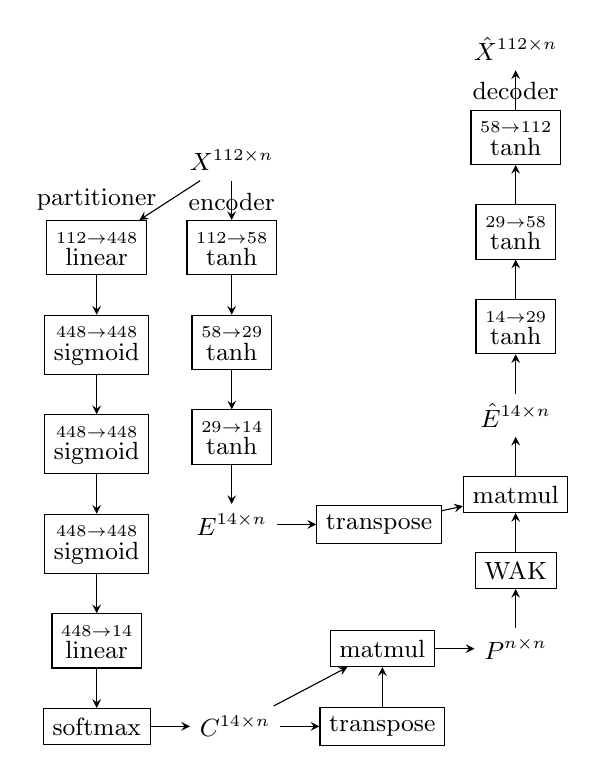
\begin{tikzpicture}[
    node distance = 5mm and 5mm,
    punkt/.style = {rectangle, draw},
    pil/.style = {black, -stealth},
    font=\small
    ]

  %\node[punkt] (preprocessing) {preprocessing} ;
  \node[] (X) {$X^{112 \times n}$} ;
  \node[punkt,label=above:encoder] (e1) [below=of X] {$\tanhl^{112 \to 58}$} ;
  \node[punkt] (e2) [below=of e1] {$\tanhl^{58 \to 29}$} ;
  \node[punkt] (e3) [below=of e2] {$\tanhl^{29 \to 14}$} ;
  \node[] (E) [below=of e3] {$E^{14 \times n}$} ;
  \node[punkt] (Etranspose) [right=of E] {transpose} ;

  \node[punkt,label=above:partitioner] (p1) [left=of e1] {$\linear^{112 \to 448}$} ;
  \node[punkt] (p2) [below=of p1] {$\sigmoid^{448 \to 448}$} ;
  \node[punkt] (p3) [below=of p2] {$\sigmoid^{448 \to 448}$} ;
  \node[punkt] (p4) [below=of p3] {$\sigmoid^{448 \to 448}$} ;
  \node[punkt] (p5) [below=of p4] {$\linear^{448 \to 14}$} ;
  \node[punkt] (softmax) [below=of p5] {$\softmax$} ;

  \node[] (C) [right=of softmax] {$C^{14 \times n}$} ;
  \node[punkt] (Ctranspose) [right=of C] {transpose} ;
  \node[punkt] (CC) [above=of Ctranspose] {matmul} ;
  \node[] (P) [right=of CC] {$P^{n \times n}$} ;
  \node[punkt] (wak) [above=of P] {WAK} ;
  \node[punkt] (GE) [above=of wak] {matmul} ;
  \node[] (Ehat) [above=of GE] {$\hat{E}^{14 \times n}$} ;
  
  \node[punkt] (d1) [above=of Ehat] {$\tanhl^{14 \to 29}$} ;
  \node[punkt] (d2) [above=of d1] {$\tanhl^{29 \to 58}$} ;
  \node[punkt,label=above:decoder] (d3) [above=of d2] {$\tanhl^{58 \to 112}$} ;
  \node[] (Xhat) [above=of d3] {$\hat{X}^{112 \times n}$} ;

  \draw[pil] %(preprocessing) edge (X)
  (X) edge (e1)
  (e1) edge (e2)
  (e2) edge (e3)
  (e3) edge (E)
  (E) edge (Etranspose)
  (Etranspose) edge (GE)
  
  (X) edge (p1)
  (p1) edge (p2)
  (p2)edge (p3)
  (p3) edge (p4)
  (p4) edge (p5)
  (p5) edge (softmax)
  (softmax) edge (C)
  (C) edge (Ctranspose)
  (Ctranspose) edge (CC)
  (C) edge (CC)
  (CC) edge (P)
  (P) edge (wak)
  (wak) edge (GE)
  (GE) edge (Ehat)
  (Ehat) edge (d1)
  (d1) edge (d2)
  (d2) edge (d3)
  (d3) edge (Xhat);
\end{tikzpicture}


         \caption{}
         \label{fig:}
     \end{subfigure}

     \hfill
     \begin{subfigure}[b]{0.45\textwidth}
        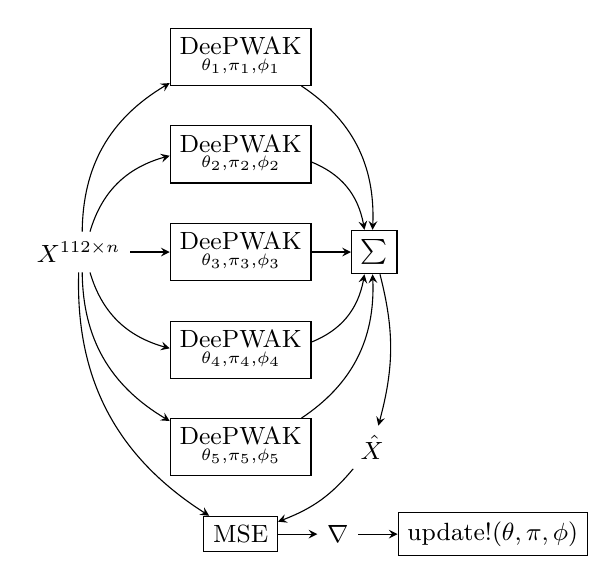
\begin{tikzpicture}[
    node distance = 5mm and 5mm,
    punkt/.style = {rectangle, draw},
    pil/.style = {black, -stealth},
    font=\small
    ]

  %\node[punkt] (preprocessing) {preprocessing} ;
  \node[] (X) {$X^{112 \times n}$} ;

  \node[punkt] (h3) [right=of X] {$\DeePWAK_{\theta_3,\pi_3,\phi_3}$} ;
  \node[punkt] (h2) [above=of h3] {$\DeePWAK_{\theta_2,\pi_2,\phi_2}$} ;
  \node[punkt] (h1) [above=of h2] {$\DeePWAK_{\theta_1,\pi_1,\phi_1}$} ;
  \node[punkt] (h4) [below=of h3] {$\DeePWAK_{\theta_4,\pi_4,\phi_4}$} ;
  \node[punkt] (h5) [below=of h4] {$\DeePWAK_{\theta_5,\pi_5,\phi_5}$} ;

  %\node[] (Xhat1) [below=of h1] {$\hat{X}_1$} ;
  %\node[] (Xhat2) [below=of h2] {$\hat{X}_2$} ;
  %\node[] (Xhat3) [below=of h3] {$\hat{X}_3$} ;
  %\node[] (Xhat4) [below=of h4] {$\hat{X}_4$} ;
  %\node[] (Xhat5) [below=of h5] {$\hat{X}_5$} ;

  \node[punkt] (sum) [right=of h3] {$\sum$} ;
  \node[] (Xhat) [right=of h5] {$\hat{X}$} ;
  \node[punkt] (loss) [below=of h5] {MSE} ;
  \node[] (grad) [right=of loss] {$\nabla$} ;
  \node[punkt] (update) [right=of grad] {$\mathrm{update!}(\theta,\pi,\phi)$} ;
  
  \draw[pil] %(preprocessing) edge (X)

  (X) edge[bend left=30] (h1)
  (X) edge[bend left=30] (h2)
  (X) edge (h3)
  (X) edge[bend right=30] (h4)
  (X) edge[bend right=30] (h5)

  (h1) edge[bend left=30] (sum)
  (h2) edge[bend left=30] (sum)
  (h3) edge (sum)
  (h4) edge[bend right=30] (sum)
  (h5) edge[bend right=30] (sum)

  (sum) edge[bend left=15] (Xhat)
  (Xhat) edge[bend left=15] (loss)
  (X) edge[bend right=30] (loss)
  (loss) edge (grad)
  (grad) edge (update);
\end{tikzpicture}

  

         \caption{}
         \label{fig:}
     \end{subfigure}
     
     %\vspace{1cm}
     %\begin{subfigure}[t]{0.45\textwidth}
     %   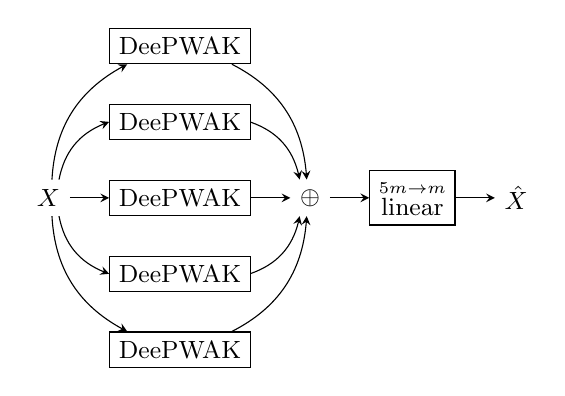
\begin{tikzpicture}[
    node distance = 5mm and 5mm,
    punkt/.style = {rectangle, draw},
    pil/.style = {black, -stealth},
    font=\small
    ]

  %\node[punkt] (preprocessing) {preprocessing} ;
  \node[] (X) {$X$} ;

  \node[punkt] (h3) [right=of X] {$\DeePWAK$} ;
  \node[punkt] (h2) [above=of h3] {$\DeePWAK$} ;
  \node[punkt] (h1) [above=of h2] {$\DeePWAK$} ;
  \node[punkt] (h4) [below=of h3] {$\DeePWAK$} ;
  \node[punkt] (h5) [below=of h4] {$\DeePWAK$} ;

  %\node[] (Xhat1) [below=of h1] {$\hat{X}_1$} ;
  %\node[] (Xhat2) [below=of h2] {$\hat{X}_2$} ;
  %\node[] (Xhat3) [below=of h3] {$\hat{X}_3$} ;
  %\node[] (Xhat4) [below=of h4] {$\hat{X}_4$} ;
  %\node[] (Xhat5) [below=of h5] {$\hat{X}_5$} ;

  %\node[punkt] (sum) [right=of h3] {$\sum$} ;
  \node[] (concat) [right=of h3] {$\oplus$} ;
  \node[punkt] (linear) [right=of concat] {$\linear^{5m \to m}$} ;
  \node[] (Xhat) [right=of linear] {$\hat{X}$} ;
  %\node[punkt] (loss) [below=of h5] {MSE} ;
  %\node[] (grad) [right=of loss] {$\nabla$} ;
  %\node[punkt] (update) [right=of grad] {$\mathrm{update!}(\theta,\pi,\phi)$} ;
  
  \draw[pil] %(preprocessing) edge (X)

  (X) edge[bend left=30] (h1)
  (X) edge[bend left=30] (h2)
  (X) edge (h3)
  (X) edge[bend right=30] (h4)
  (X) edge[bend right=30] (h5)

  (h1) edge[bend left=30] (concat)
  (h2) edge[bend left=30] (concat)
  (h3) edge (concat)
  (h4) edge[bend right=30] (concat)
  (h5) edge[bend right=30] (concat)

  (concat) edge (linear)
  (linear) edge (Xhat) ;
  %(sum) edge[bend left=15] (Xhat) ;
  %(Xhat) edge[bend left=15] (loss) 
  %(X) edge[bend right=30] (loss)
  %(loss) edge (grad)
  %(grad) edge (update);
\end{tikzpicture}

  

     %    \caption{}
     %    \label{fig:}
     %\end{subfigure}

     %\hfill
     %\begin{subfigure}[t]{0.45\textwidth}
     %  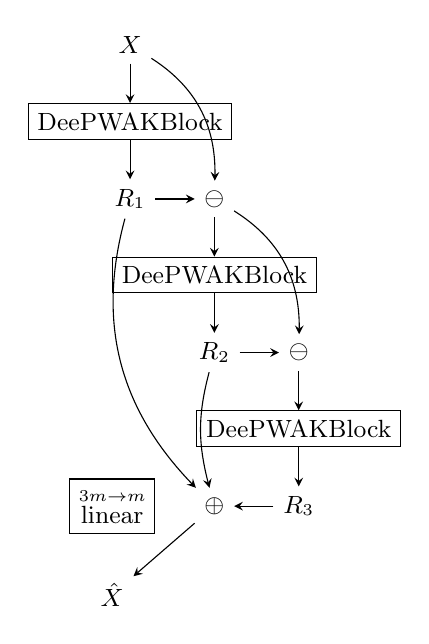
\begin{tikzpicture}[
    node distance = 5mm and 5mm,
    punkt/.style = {rectangle, draw},
    pil/.style = {black, -stealth},
    font=\small
    ]

  \node[] (X) {$X$} ;
  \node[punkt] (b1) [below=of X] {DeePWAKBlock} ;
  \node[] (R1) [below=of b1] {$R_1$} ;
  \node[] (diff1) [right=of R1] {$\ominus$} ;

  \node[punkt] (b2) [below=of diff1] {DeePWAKBlock} ;
  \node[] (R2) [below=of b2] {$R_2$} ;
  \node[] (diff2) [right=of R2] {$\ominus$} ;
  
  \node[punkt] (b3) [below=of diff2] {DeePWAKBlock} ;
  \node[] (R3) [below=of b3] {$R_3$} ;
  %\node[] (diff3) [right=of R3] {$\ominus$} ;
  
  \node[] (concat) [left=of R3] {$\oplus$} ;
  \node[punkt] (linear) [left=of concat] {$\linear^{3m \to m}$} ;
  \node[] (Xhat) [below=of linear] {$\hat{X}$} ;

  \draw[pil]
  (X) edge (b1)
  (b1) edge (R1)
  (R1) edge (diff1)
  (X) edge[bend left=30] (diff1)

  (diff1) edge (b2)
  (b2) edge (R2)
  (R2) edge (diff2)
  (diff1) edge[bend left=30] (diff2)
  
  (diff2) edge (b3)
  (b3) edge (R3)
  %(R3) edge (diff3)
  %(diff2) edge[bend left=30] (diff3)

  (R1) edge[bend right=30] (concat)
  (R2) edge[bend right=15] (concat)
  (R3) edge (concat)
  (concat) edge (Xhat) ;
\end{tikzpicture}

  

     %  \caption{}
     %  \label{fig:}
     %\end{subfigure}
     
     \caption{(a) Architecture of one DeePWAK head. (b) Training loop for DeePWAK block.}
     \label{fig:}
\end{figure}


\section{Results}

\subsection{Multihead DeePWAK learns sparse representations}

\section{Discussion}

\printbibliography

\end{document}
